Data were generated by training an auto-encoder neural network.
\begin{itemize}\compresslist
\item Two areas specified to be \A and \B selective.
\item One area placed between systematic input and output units.
\item Categorization is possible based on either region, but the information is represented very differently.
\end{itemize}

\begin{center}
{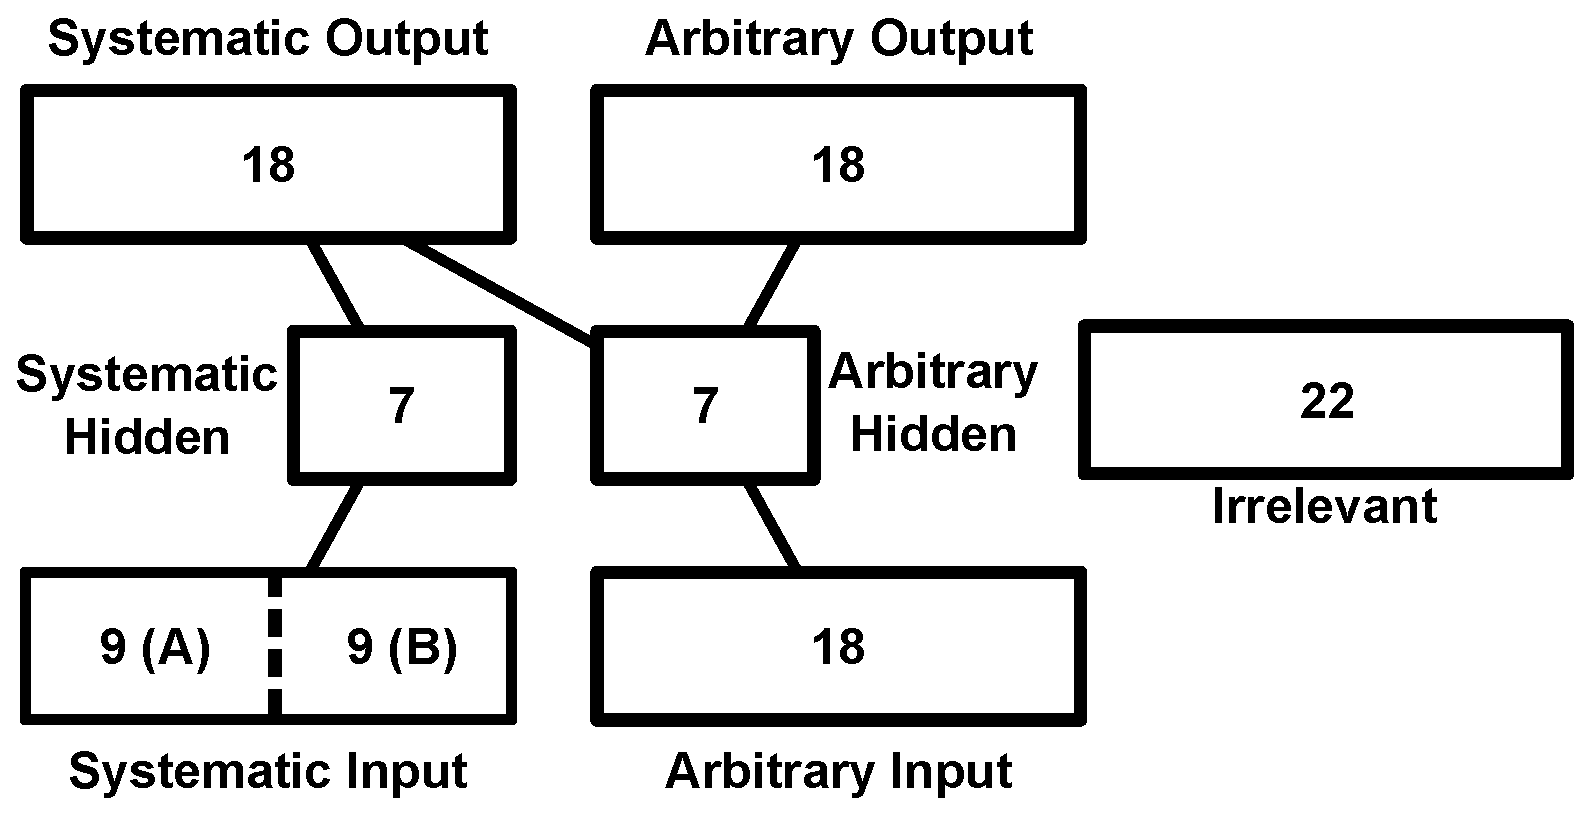
\includegraphics[width=0.65\textwidth]{model_outline.eps}}
{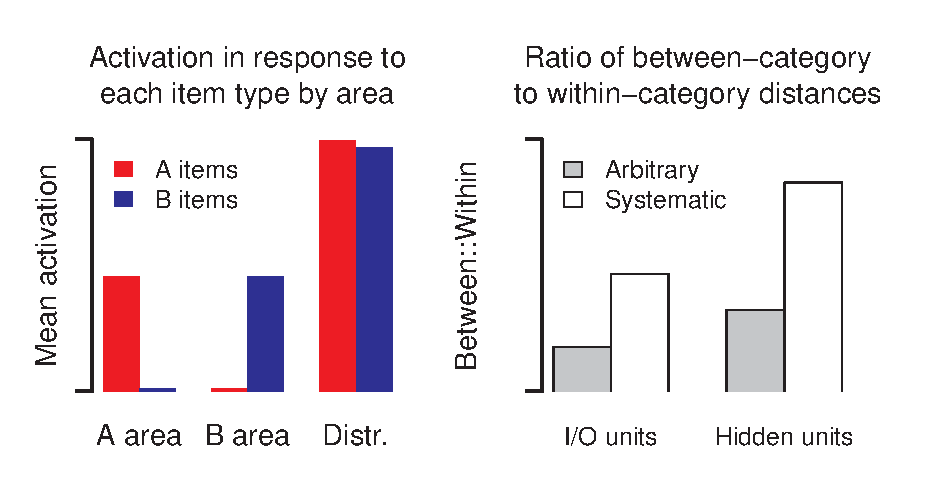
\includegraphics[width=0.75\textwidth]{activation_vs_distance.eps}}
\end{center}

{\bf Methods vary in their representational assumptions, and will label different patterns of data as ``important''.} We explore this by applying a range of methods to these data, to obviate the consequences of these assumptions.